% !TEX encoding = UTF-8 Unicode
\documentclass[a4paper, 12pt]{article}
\usepackage{graphicx}
\usepackage{amsmath}
\usepackage[brazil]{babel}
\usepackage[utf8]{inputenc}

\author{Seu nome}
\title{}

\linespread{1.5}


\begin{document}
%Capa
\begin{center}
\textbf{MINISTÉRIO DA DEFESA}\\
\textbf{EXÉRCITO BRASILEIRO}\\
\textbf{DEPARTAMENTO DE CIÊNCIA E TECNOLOGIA}\\
\textbf{INSTITUTO MILITAR DE ENGENHARIA}\\
\textbf{Programa de Engenharia de Defesa / PGED}

\vspace{2.5cm}

\begin{large}
\textbf{Proposta de Tema de Dissertação de Mestrado
\\Curso: Mestrado em Engenharia de Defesa}

\vspace{1.5cm}

\textbf{Título: Opções na contracapa!!!!!}

\vspace{1.5cm}


\textbf{Orientador: Paulo Fernando Ferreira Rosa, Ph.D}

\end{large}

\vspace{1.5cm}

\textbf{Aluno: Bruno da Silva Giovanini (ED 14106)}


\vspace{2cm}

\begin{small}
Data de Apresentação no PGED:\\
Rio de Janeiro, XX de fevereiro de 2015
\end{small}

\end{center}


%Título
\newpage
\begin{large}
\section*{Título da Dissertação}
\textbf{Título da Tese:}\\
\textbf{Sistemas de Defesa: Controle de um quadricóptero com desvio de obstáculos automático em tempo real}\\

\noindent\textbf{Sistemas de Defesa: Uma abordagem para desvios de obstáculos no auxílio do controle de um quadricóptero em tempo real}\\
 

\noindent\textbf{Título da Capa:}\\
\textbf{???????????}\\

\noindent\textbf{Área de Concentração:}\\
Engenharia de Defesa\\

\noindent\textbf{Linha de Pesquisa:}\\
Mecatrônica e Sistemas de Armas\\
\end{large}

%Desenvolvimento do Texto
\newpage

\abstract

A utilização de veículos aéreos para missões em ambientes fechados e restritos, tanto militares quanto civis, vem aumentando e os desafios envolvidos em seu controle estão atraindo as comunidades científica e industrial. Com isso, o desvio de obstáculos de forma automática ganha importância nesse cenário, dada a dificuldade de controle e o risco de colisão envolvido no manuseio destes veículos. Este trabalho propõe uma abordagem para controle do desvio de obstáculos de um quadricóptero de forma automática permitindo que sua operação mantenha o foco na missão global e evitar, assim, possíveis acidentes. 
O método consiste em evitar colisões estimando constantemente sua trajetória com base na dinâmica, estado atual, controle corrente e sensores ultrassônicos de distância. A validação desta proposta será realizada em ambiente simulado \textit{hardware-in-the-loop} e posteriormente, com o embarque do sistema em um quadricóptero para voo em campo.

 
\newpage

\section{Introdução}

A utilização de robôs voadores tanto em aplicações militares quanto civis vem aumentando e os desafios envolvidos em seu desenvolvimento estão atraindo as comunidades científica e industrial. Graças a isso, os veículos aéreos não tripulados (VANTs) têm se tornado cada vez mais populares. Tarefas como monitoramento de áreas alagadas, resgates em regiões de difícil acesso e inspeção de equipamentos perigosos, são aplicações que tornam os VANT's cada vez mais presentes no nosso cotidiano.

\subsection{Motivação}

Recentes avanços em processadores de baixo consumo de energia e na miniaturização dos componentes eletrônicos e sensores estão expandindo o campo de utilização dos VANT's para ambientes mais restritos. Veículos aéreos não tripulados de menor escala com decolagem e aterrissagem vertical, também chamados de Mini-VTOL (\textit{Mini vertical taking-off and landing}) ou simplesmente VTOL, apresentam muitas vantagens em ambientes desse tipo, devido sua flexibilidade e agilidade quando em movimento. Essas habilidades tornam possível sua utilização em tarefas como busca e resgate em prédios e inspeção de áreas fechadas sem colocar outras vidas em risco. Porém, áreas restritas aumentam o risco do choque entre o robô e os itens ali contidos, dado o espaço limitado para sobrevoo. Nesse contexto, um mecanismo de controle que evite colisões contra obstáculos se torna importante para aumentar a segurança do voo e é o objeto dessa proposta. Acredita-se que, essa solução irá expandir o número dos possíveis campos de atuação de VTOL's para tarefas ainda consideradas perigosas, como sobrevoo em áreas com equipamentos críticos e sensíveis.



\subsection{Objetivo}

O propósito desse trabalho é controlar o desvio de obstáculos de um VTOL, um quadricóptero, de forma automática permitindo que sua operação mantenha o foco na missão global e evitar, assim, possíveis acidentes. Especificamente, propomos um método que consiste em estimar continuamente a trajetória futura do veículo, dada sua dinâmica, seu estado atual e o \textit{input} de controle corrente. Desta forma, facilitar o controle de voo contribuindo para a segurança de voos desta plataforma. 

%Além disso, através das medidas de sensores de distância embarcados, realizar uma comparação com a trajetória e identificar possíveis colisões. Se uma colisão é iminente, um novo controle é selecionado e o controle do operador é minimizado até que não exista possibilidade de colisão.


\subsection{Estrutura da Proposta}

A continuidade desta proposta está estruturada como segue. Inicialmente é discutida a revisão de literatura na seção \ref{sec:rev}. Após, os tópicos tutoriais relacionados estão descritos na seção \ref{sec:tutoriais}. Uma descrição do problema em questão é abordado na seção \ref{sec:prob} e metodologia proposta é descrita na seção \ref{sec:meto}. Em seguida, o cronograma de execução é mostrado na seção \ref{sec:crono}, a viabilidade da pesquisa na seção \ref{sec:viabilidade} e os resultados esperados na seção \ref{sec:resultados}. Por fim, na seção \ref{sec:conclusao}, é feita uma conclusão sobre o potencial dessa proposta. 

\newpage

\section{Revisão de Literatura}
\label{sec:rev}

Nos últimos anos, veículos aéreos não tripulados receberam uma maior atenção da comunidade de robótica. Muitos autores focaram na modelagem e no controle destes veículos \cite{Ye2006},  com especial destaque para os quadricópteros \cite{Altug2002}. Nesse contexto, estudos abrangentes sobre a configuração da plataforma, metodologias de modelagem, modelagem compreensiva não linear, os efeitos aerodinâmicos, identificação e simulação de um quadricóptero foram realizados \cite{Zhang2014} \cite{Gibiansky2010}. Por ser considerado um sistema complexo não linear, técnicas para controle de quadricópteros são também amplamente estudadas. \cite{Salih2010} desenvolveu um controle PID para um quadricóptero para obter estabilidade em voo. Por outro lado, \cite{Nicol2008}, propôs uma rede neural adaptativa para estabilizar o quadricóptero levando em consideração erros de modelagem e distúrbios do vento.

A partir de um modelo conhecido, diversas são as aplicações em estudo. Para a maioria, como navegação autônoma, tarefas multiagentes e desvio de obstáculos, a estimação do estado do veículo é considerado um grande desafio \cite{Achtelik2009}. Quando se trata de ambientes \textit{indoors}, a visão computacional, que utiliza-se de câmeras e processamento de imagem para estimação, é uma das linhas de pesquisa sobre o problema \cite{Shen2013} \cite{Blosch2010} \cite{Shen2013a}. Outra linha utiliza-se de sensores estereoceptivos para tal tarefa, como ultra-som \cite{Roberts2007} e laser \cite{Grzonka2012}. Já para ambientes \textit{outdoors}, torna-se possível a utilização do Sistema de Posicionamento Global (GPS) e alguns trabalhos que utilizam essa tecnologia foram desenvolvidos, como  \cite{Hoffmann2004} e \cite{Wendel2006}.

%A plataforma Parrot Ar.Drone, 

Quando se fala especificamente sobre desvio de obstáculos em tempo real, esse campo é bastante explorado em robótica. Para resolver essa questão, várias são as abordagens que vem sido adotadas. Dentre elas, os métodos baseados em campos potenciais artificiais,  onde sensores de distância são usados e suas medidas tratadas como vetores de repulsão de forças \cite{Bouktir2008}, \cite{Nieuwenhuisen2013} e \cite{Borenstein1989}; o método de janelas dinâmicas, que incorpora a dinâmica do robô ao problema através da redução do espaço de busca das possíveis velocidades alcançáveis em um curto período de tempo (janela dinâmica) \cite{Fox1997} \cite{Saranrittichai2013}; método de obstáculos com velocidade, que define um conjunto de velocidades possíveis que resultaria em uma colisão entre o robô e um obstáculo se movendo em uma certa velocidade \cite{Fiorini1998} \cite{Claes2012} \cite{Berg2012}; método de estados de colisões inevitáveis, considerado um estado em que uma colisão eventualmente irá ocorrer, independente da trajetória a ser estabecida e que leva em conta a dinâmica tanto do robô quanto dos obstáculos, fixos ou móveis \cite{Fraichard2004}; dentre outros.   

Um trabalho semelhante ao aqui proposto foi realizado por \cite{Israelsen}, porém o ambiente e a posição dos obstáculos já eram previamente conhecidos e geometricamente pré-programados, não sendo utilizado sensores de distância. \cite{Grzonka2012} também desenvolveu um quadricóptero totalmente autônomo em ambiente \textit{indoor}, utilizando para o desvio de obstáculos o sensor de varredura a laser em miniatura Hokuyo-URG, considerado o menor e mais leve sensor a laser disponível comercialmente. Já \cite{Becker2012} utilizou cinco sensores ultrassônicos para tal. Porém, tanto \cite{Grzonka2012} quanto \cite{Becker2012} utilizaram plataformas desenvolvidas e testadas previamente em laboratório por alguns anos, tendo em mãos modelagens dos veículos já bem definidas.



\newpage

\section{Tópicos Tutoriais}
\label{sec:tutoriais}

Nessa seção serão abordados os principais aspectos teóricos envolvidos nessa proposta. Inicialmente, 
o quadricóptero, que é a plataforma de voo a ser aqui estudada, será descrita juntamente com sua dinâmica de voo. Após, os dispositivos embarcados e suas contribuições para o controle do voo e, por fim, o controle PID e sua utilização para o controle de quadricópteros.

\subsection{O Quadricóptero}

\cite{Salih2010} define o quadricóptero como um veículo voador com quatro rotores com decolagem e aterrissagem vertical. Por sua vez, \cite{Gibiansky2010} define quadricóptero como uma classe de helicópteros com quatro rotores girando rapidamente para empurrar o ar para baixo e criar uma força para mantê-lo elevado e posicionados nas extremidades de um corpo quadrado. A Figura \ref{fig:quad} ilustra a plataforma Parrot ArDrone 2.0, um quadricóptero bastante estudado e utilizado na comunidade de robótica.

\begin{figure}[h]
	\centering
		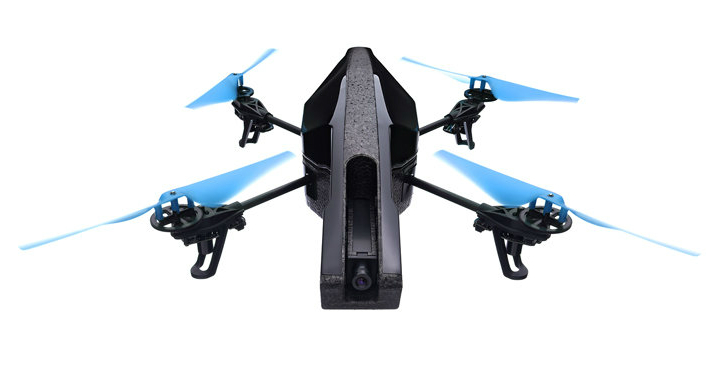
\includegraphics[scale=0.4]{img/parrot_drone.jpg}
	\caption{Plataforma Parrot Ardrone 2.0. Fonte \cite{ardrone}}
	\label{fig:quad}
\end{figure}

\noindent\textbf{Dinâmica de voo}

O objetivo da dinâmica de voo é manter a estabilidade do eixo central do quadricóptero,  controlando os quatro rotores que trabalham de forma independente. Esse processo é considerado complexo e precisa de apoio eletrônico para a execução \cite{Gibiansky2010}. A controladora de voo é responsável por controlar a intensidade das rotações individualmente, de acordo com o movimento preterido. Um dos possíveis controles realizados pela controladora de voo é o PID que será abordado na seção \ref{subsec:PID}.

O quadricóptero é um sistema não linear, fortemente acoplado com seis graus de liberdade, onde três são movimentos lineares (x,y,z) e os outros três angulares ($\phi$,$\theta$,$\psi$). Porém, possui apenas quatro atuadores, sendo considerado então um sistema \textit{underactuated}, com dois movimentos lineares (x,y) dependentes dos movimentos angulares ($\phi$,$\theta$). As forças e momentos atuando no quadricóptero são produzidos pelas hélices ligadas aos rotores. Dois rotores rodam no sentido horário e dois no sentido anti-horário dispostos de forma à balancear o torque total do sistema \cite{Mian2008}. A Figura \ref{fig:diag quad} (esquerda) mostra a disposição dos motores e suas orientações de funcionamento. Já a Figura \ref{fig:diag quad} (direita)  mostra o diagrama do corpo e os eixos do quadricóptero.

Na Figura \ref{fig:diag quad}(direita), \textit{l} representa a distância entre cada rotor e o centro, $\phi$, $\theta$ e $\psi$ representam os ângulos de Euler em relação aos eixos x, y e z, chamados de rolagem, afagem e guinada, respectivamente. $T_i$ (i = 1, 2, 3, 4) é a força de empuxo produzida por cada hélice e cada seta circular ao redor de $T_i$ indica o sentido de rotação daquele rotor. O referencial inercial é denotado por E(X,Y,Z) e o referencial do corpo do quadricóptero é denotado por B(x,y,z). 

\begin{figure}[h]
	\centering
		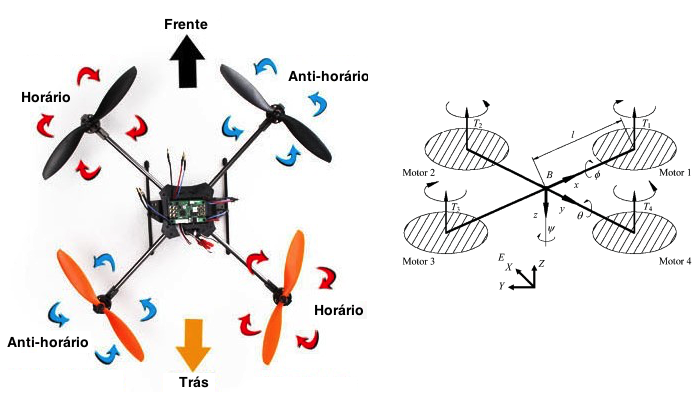
\includegraphics[scale=0.5]{img/diagrama_quadricoptero.png}
	\caption{Estrutura e orientação dos motores (esquerda) e as forças e momentos atuando no quadricóptero (direita). Fontes \cite{quadblog} e \cite{Mian2008}.}
	\label{fig:diag quad}
\end{figure}

O aumento ou a diminuição da velocidade dos quatro rotores na mesma proporção irá gerar um movimento vertical. Quando os motores do par (1,3) operam independentemente e o par (2, 4) mantém a mesma velocidade, o ângulo de inclinação do par (1,3), em relação ao eixo y (afagem), poderá ser controlado e, indiretamente, executará um movimento ao longo de seu eixo. Da mesma forma, a operação independente do par de motores (2,4), enquanto (1,3) com velocidade constante, poderá controlar o ângulo de rolagem em relação ao eixo x e um controle indireto do movimento ao longo do seu eixo também será feito. E, por fim, se ambos os pares possuírem velocidades independentes, o ângulo de guinada, em relação ao eixo z, poderá ser controlado. Dessa forma, o quadricóptero apresenta seis graus de liberdade e pode ser mover com agilidade. 

\subsection{Sistemas Embarcados de Navegação}

Navegação inercial é o processo pelo qual se adquirem informações sobre a posição, velocidade e atitude de um veículo com relação a um dado referencial, utilizando informações fornecidas por sensores inerciais tais como acelerômetros e giroscópios. Medindo-se as acelerações e velocidades angulares de um corpo, torna-se possível calcular as mudanças de velocidade, posição e atitude através de sucessivas integrações numéricas \cite{Adalberto2009}.

A unidade de medida inercial, ou IMU, é o componente eletrônico onde são montados os sensores inerciais, sendo três acelerômetros, que fornecem as medidas das componentes da aceleração linear (x,y,z), e três giroscópios, sensores que fornecem as componentes da velocidade angular (por exemplo, arfagem, rolagem e guinada). Já a unidade de processamento é o componente responsável por processar as medidas dos sensores inerciais. As velocidades lineares e as posições são obtidas a partir da integração dos sinais dos acelerômetros, enquanto que a integração dos sinais dos giroscópios fornece a atitude do veículo.  A Figura \ref{fig:imuStrap} ilustra a estrutura de um Sistema de Navegação Inercial acoplado a um veículo, composta por três giroscópios, três acelerômetros (x,y,z) e uma unidade de processamento (CPU) à esquerda e os movimentos gerados no quadricóptero à direita.

\begin{figure}[h]
	\centering
		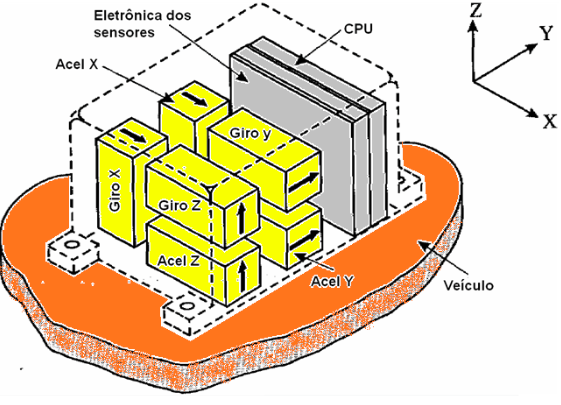
\includegraphics[scale=0.6]{img/imuStrap.png}
	\caption{Estrutura do Sistema de Navegação acoplada ao veículo (esquerda) e os movimentos gerados no quadricóptero (direita). Fonte \cite{Adalberto2009}}
	\label{fig:imuStrap}
\end{figure}

Magnetômetros podem ser incluídos em IMUs, permitindo uma melhor performance de cálculos de orientação em sistemas AHRS (do inglês, \textit{Attitude Heading Reference System}). Um sistema AHRS é composto de sensores que fornecem a orientação e atitude de uma aeronave. A principal diferença entre uma IMU e um AHRS é a adição de um sistema de processamento embarcado em um AHRS que fornece soluções de atitude e orientação, contra a IMU que apenas fornece os dados do sensor \cite{Angonese2013}.

A Figura \ref{fig:imuVANTIME} demonstra o protótipo de uma IMU desenvolvida para o projeto VANT-IME. No hardware desenvolvido foram utilizados, um acelerômetro que mede a aceleração do veículo e um giroscópio de três eixos para complementar o acelerômetro, obtendo-se assim, informações de velocidade angular em altas frequências, o que se faz necessário para estabilização de aeronaves movendo-se em alta velocidade. Entretanto, devido a erros de deriva dos giroscópios, erros de integração e ao ruído, a utilização de um magnetômetro se faz necessária, pois permite a medição do campo magnético no qual está inserido. As informações de todos os sensores são lidas, filtradas e então processadas para a estimação da atitude da aeronave \cite{Paixao2011}. As Figuras \ref{fig:imuVANTIME}a,  \ref{fig:imuVANTIME}b,  \ref{fig:imuVANTIME}c ilustram as leituras dos sensores inerciais e a Figura \ref{fig:imuVANTIME}d demostra o gráfico resultante após a filtragem e processamento das leituras dos sensores individuais.

\begin{figure}[h]
	\centering
		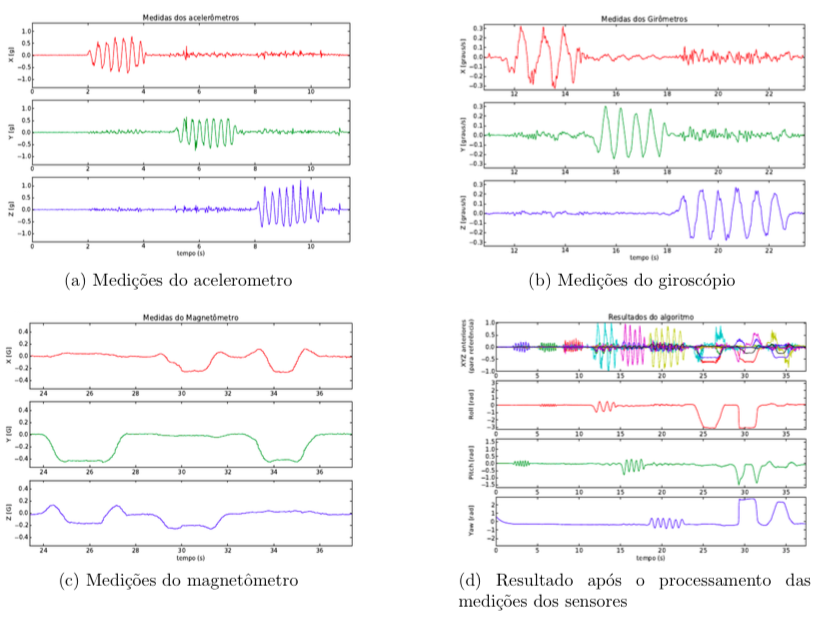
\includegraphics[scale=0.5]{img/imu_VANTIME.png}
	\caption{Gráfico das medições dos sensores inerciais da IMU do VANT-IME. Fonte \cite{Paixao2011}}
	\label{fig:imuVANTIME}
\end{figure}

\noindent\textbf{Acelerômetros e Giroscópios}

Acelerômetros são sensores que fornecem a medida e a força específica que atua no veículo, que é a resultante das ações da aceleração inercial e da aceleração da gravidade. Portanto, a partir da medida da força específica e do modelo do campo gravitacional da Terra, determina-se a aceleração linear, informação que é integrada para a determinação da velocidade e posição do veículo.

Giroscópios fornecem a medida da velocidade angular. Este dado é utilizado para a determinação da atitude do veículo. Já está na terceira geração. Esta, devido suas características de menor custo e volume, possibilitou sua utilização em grande escala em veículos de pequeno porte. Porém, sua exatidão é menor quando comparado às gerações anteriores. É formado por sensores baseados na tecnologia MEMS (\textit{Micro Electro Mechanical Systems}) que consistem em placas de cerâmicas vibrantes que utilizam Força de Coriolis para medir a taxa independente da aceleração \cite{Adalberto2009}.

\subsection{Controle PID e quadricópteros}

\label{subsec:PID}

Um controle PID é um método comum para controlar robôs e a sua utilidade está na aplicabilidade geral na maioria dos sistemas de controle, principalmente quando o modelo matemático de planta é complexo e não conhecido \cite{Ogata2003}. É um sistema de controle fechado que reage a mudanças no ambiente, que são captadas por sensores, e se baseia na constante sintonia das entradas para obter a saída esperada \cite{Kingdom}.  

O algoritmo de cálculo do controle PID envolve três parâmetros constantes: o valor proporcional (P), o valor integral (I) e o valor derivativo (D) e serão descritos a seguir:

\begin{itemize}
\item
Valor proporcional - É tipicamente o erro. Ele é usualmente a distância que o robô deve viajar, ou a temperatura que se queira alcançar. Se o robô está na posição A, mas quer estar na posição B, então o valor proporcional P é $A - B$.
\item
Valor integral - É o acúmulo dos erros passados no tempo (t). Por exemplo, se o robô está continuamente fora da média por uma certa quantidade de tempo, o valor I irá tratar isso. Supondo que em $t_1$ o erro era A, em $t_2$ o erro era B e em $t_3$ o erro era C. o valor integral I seria $A/t_1 + B/t_2 + C/t_3$.
\item
Valor derivativo - É a mudança do erro no tempo (t). Por exemplo, se o erro era C e, depois do tempo t, passou a ser D, o valor derivativo D é $(C-D)/t$. Normalmente, o contador de tempo da microcontroladora é utilizado para medir esse tempo. Além disso, D é utilizado para predizer mudanças futuras baseando-se na taxa mudança atual.
\end{itemize}

A soma ponderada desses três termos é usada para ajustar o processo através de um elemento de controle, como uma válvula ou como o controle da quantidade de energia aplicada no sistema. O peso é atribuído através de uma constante K denominada ganho e tem o papel de ajustar os valores P, I e D. Ou seja, cada termo P, I e D possui o seu ganho associado e a equação básica de controle é dada pela fórmula \ref{eq:equacaoPID}. 

\begin{equation}
	\centering
		P*K_p + I*K_i + D*K_d	
	\label{eq:equacaoPID}
\end{equation}

A atuação do ganho no desempenho do sistema de controle PID pode ser visualizado na Figura \ref{fig:ganhoPID}, onde a linha azul indica o sinal de referência e as demais linhas indicam diferentes comportamentos com a variação dos ganhos $K_p$, $K_i$ e $K_d$. Um menor tempo de estabilização é normalmente desejável \cite{Kingdom}.  

\begin{figure}[h]
	\centering
		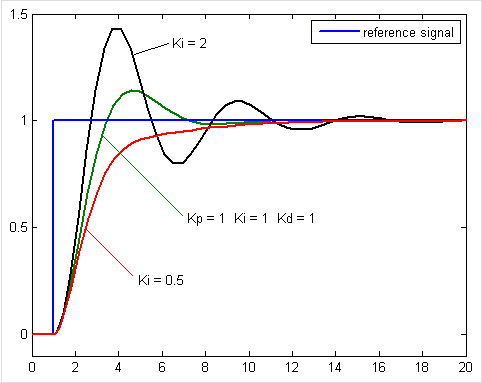
\includegraphics[scale=0.5]{img/ganho_PID.png}
	\caption{Desempenho do sistema para diferentes ganhos $K_p$, $K_i$ e $K_d$. Fonte \cite{Kingdom}}
	\label{fig:ganhoPID}
\end{figure}
 
\noindent\textbf{PID em quadricópteros}

A maioria dos quadricópteros utilizam PID para estabilização e permitem que o usuário altere os parâmetros para ajustar a performance \cite{Liang}. A Figura \ref{fig:PIDquad} ilustra o esquema de controle PID de um quadricóptero para a estabilização. Basicamente, o \textit{feedback} é obtido através dos sensores do quadricóptero que são avaliados em conjunto com o movimento pretendido pelo piloto através do controle PID e, após, passado ao atuador como comando para os motores. 

\begin{figure}[h]
	\centering
		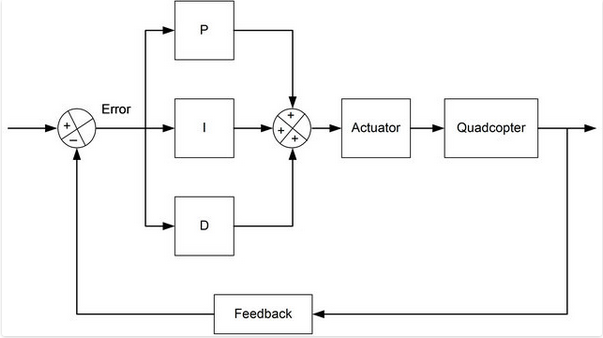
\includegraphics[scale=0.5]{img/PID_quad_geral.png}
	\caption{Controle PID de um quadricóptero. Fonte \cite{Liang}}
	\label{fig:PIDquad}
\end{figure}


Geralmente, segundo \cite{Liang}, existem ao todo três controles PID's, um para cada eixo ($\phi$,$\theta$,$\psi$) e a alteração dos valores dos ganhos ($K_p$, $K_i$ e $K_d$) de cada eixo acarretará em mudanças na reação do quadricóptero quando sujeito a interferências externas. A Figura \ref{fig:PIDaxis} ilustra a estrutura do controle PID de um eixo.

%\begin{itemize}
%\item
%$K_p$ - O quadricóptero pode voar de forma estável somente com esse ganho. Ele determina qual é mais importante, o controle humano ou os valores medidos pelo giroscópio. Quanto maior o coeficiente, mais sensível e reativo ele será para mudanças de ângulos. Se muito pequeno, mais lento e difícil de mantê-lo estável.
%\item
%$K_i$ - Pode aumentar a precisão da posição angular. O tempo de reação à uma alteração do ângulo de inclinação é afetada.
%\item
%$K_d$ - Permite ao quadricóptero alcançar a atitude desejada mais rapidamente. Ele amplifica a ação do usuário. 

%\end{itemize}

\begin{figure}[h]
	\centering
		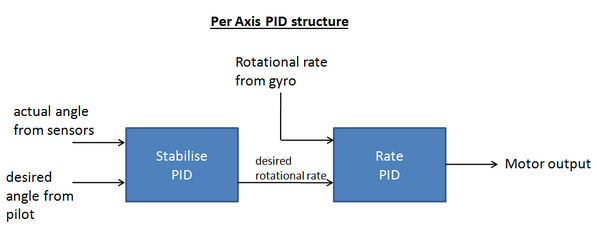
\includegraphics[scale=0.8]{img/PID_quad_axis.png}
	\caption{Controle PID por eixo. Fonte \cite{Liang}}
	\label{fig:PIDaxis}
\end{figure}



\newpage

\section{O Problema: Segurança em voo para quadricóptero}
\label{sec:prob}

O problema a ser tratado consiste em evitar que o quadricóptero se choque durante sua navegação através de um método que estima continuamente a trajetória futura do veículo, dada sua dinâmica, seu estado atual e o \textit{input} de controle. Para isso, variações no controle são realizadas baseadas em estimativas futuras de colisão. A formulação matemática do problema é descrita a seguir.


%Para isso, torna-se necessário a estimação de sua posição futura, a avaliação de uma possível colisão e a geração de variações de controle a fim de obter um deslocamento seguro. 

\noindent\textbf{Formulação do Problema}

Considerando um quadricóptero como um robô com uma dinâmica não linear genérica em um espaço arbitrário, $\mathcal{X} \subset R^{n}$ o seu espaço de estados e $\mathcal{U} \subset R^{n}$ o espaço do \textit{input} de controle. Em tempo contínuo, a dinâmica do robô é uma função em $\mathbf{f} \in \mathcal{X} \times \mathcal{U} \times R \rightarrow R^{n}$ e é dada pela relação \ref{eq:equacaoDinProb}:

\begin{equation}
\centering
\dot{\mathbf{x}} = \mathbf{f}(\mathbf{x}(t),\mathbf{u}(t),t)  
\label{eq:equacaoDinProb}
\end{equation}

\noindent onde $t$ é o tempo, $\mathbf{x}(t)$ é o estado do robô no tempo $t$ e $\mathbf{u}(t)$ é o \textit{input} de operação no tempo $t$. Consequentemente, dado um estado inicial $\mathbf{x_0} = \mathbf{x}(0)$ e uma constante de \textit{input} de operação $\mathbf{u}$, o estado do robô em um instante $t > 0$ é dado pela relação \ref{eq:equacaoPosProb}:
 

\begin{equation}
\centering
\mathbf{x} = \mathbf{g}(\mathbf{x},\mathbf{u},t)  
\label{eq:equacaoPosProb}
\end{equation}

\noindent onde $\mathbf{g} \in \mathcal{X} \times \mathcal{U} \times R \rightarrow \mathcal{X}$ representa a solução da equação diferencial \ref{eq:equacaoDinProb}.

Porém, quando se considera um ambiente repleto de obstáculos, o espaço de estados do robô se restringe à posições não ocupadas por eles. Define-se então $\mathcal{O} \subset R^3$, como a subárea do espaço $R^n$ de movimentos possíveis do robô ocupada por obstáculos e as regiões que estão escondidas por eles quando vistas pelo estado corrente do robô. Além disso, $\mathcal{R}(x)$, como a subárea ocupada pelo robô no estado $x \in \mathcal{X}$. Assim, o problema passa a ser definido como identificar a menor variação necessária  $\Delta\mathbf{u} \in \mathcal{U}$ sobre o controle de operação $\mathbf{u}$, dado o atual estado $\mathbf{x}$ do robô, a fim de que se evite uma colisão com algum obstáculo em qualquer momento até se alcançar um período previamente definido $\tau \in R$ conforme a relação \ref{eq:equacaoProb}:

\begin{equation}
\begin{aligned}
\text{min: }& \Delta\mathbf{u} \\
\text{Sujeito a: }& \forall t \in [0,\tau], \mathcal{R}(\mathbf{g}(\mathbf{x}, \mathbf{u}+\Delta\mathbf{u}, t)) \cap \mathcal{O} = \emptyset
\end{aligned}
\label{eq:equacaoProb}
\end{equation}

%\Delta\mathbf{u^T}T\mathbf{u}

%\noindent onde $T \in R^{m \times m}$ é uma matriz positiva de pesos.

É importante notar que, caso o \textit{input} de operação $\mathbf{u}$ obedeça as restrições da equação \ref{eq:equacaoProb}, ou seja, corresponde a um deslocamento seguro, $\Delta\mathbf{u} = 0$ e nenhuma alteração do controle será realizada.

\newpage

\section{Metodologia}
\label{sec:meto}

Para resolver este problema, é proposta a seguinte metodologia. Inicialmente, obter medidas de distâncias a partir de sensores ultrassônicos, em tempo real, para detecção de obstáculos. Em seguida, confrontá-los com os dados, já filtrados, da atitude do quadricóptero obtidos da IMU para identificar colisões iminentes em uma janela de tempo pré-determinada. Em caso positivo, interceptar o comportamento gerando a menor mudança de comando possível que seja suficiente para evitar uma colisão naquela janela de tempo.

Para facilitar o entendimento, o método foi dividido em etapas que serão  descritas a seguir, juntamente com os componentes e software necessário e a estratégia de sua implementação.

\subsection{Etapas}

\label{subsec:etapas}

A Figura \ref{fig:etapasMetodo} ilustra as etapas envolvidas, onde cada cor representa um tipo de atuação e as setas indicam suas dependências. Em azul estão os responsáveis pela aquisição dos dados necessários: sensores ultrassônicos, os comandos de controle e a os sensores da IMU. Em verde, estão os processos de tratamento dos dados a fim de se obter medidas confiáveis para os módulos. Já em amarelo estão os módulos centrais para detecção de obstáculos e identificação de colisões. Por fim, em vermelho, está o controle de atitude, processo integrante da controladora de voo, que receberá comandos e os transformarão em ações do quadricóptero.   

\begin{figure}[h]
	\centering
	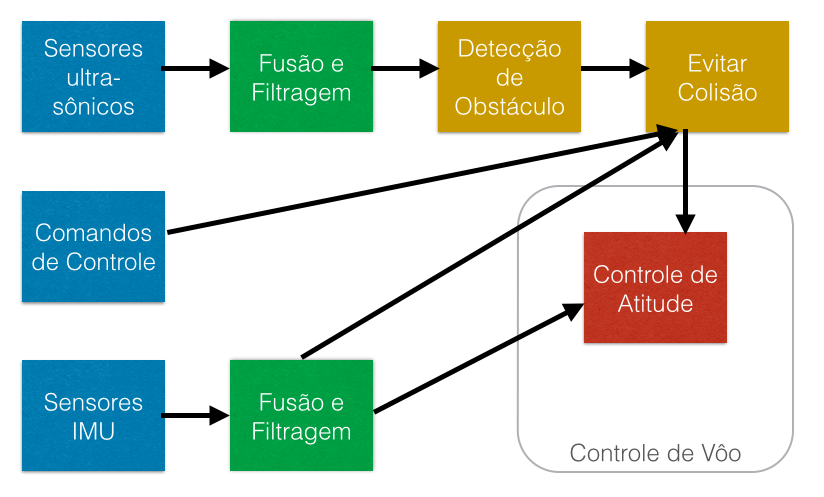
\includegraphics[scale=0.4]{img/etapasMetodo.png}
	\caption{Etapas do método}
	\label{fig:etapasMetodo}
\end{figure}

Em seguida, as etapas e uma breve descrição dos passos necessários para galgá-las no trabalho proposto:

\noindent\textbf{Sensores ultrassônicos} 
\begin{itemize}
	\item
	Definir o modelo e a quantidade de sensores ultrassônicos a serem utilizados e como dispô-los de forma a obter uma região de cobertura adequada.  
\end{itemize}

\noindent\textbf{Fusão e Filtragem dos Sensores} 
\begin{itemize}
	\item
	Definir e estudar o método que será utilizado para fusão dos sensores ultrassônicos.
\end{itemize}

\noindent\textbf{Comandos e Controle} 
\begin{itemize}
	\item
	Estudar o \textit{software development kit}, a partir daqui, chamado de SDK, de controle da plataforma de voo.  
\end{itemize}

\noindent\textbf{Sensores IMU} 
\begin{itemize}
	\item
	Verificar como obter os dados da IMU da plataforma de voo através de seu SDK.
\end{itemize}

\noindent\textbf{Fusão e Filtragem da IMU} 
\begin{itemize}
	\item
	Estudar a utilização dos dados já filtrados pela plataforma de voo.  
\end{itemize}

\noindent\textbf{Detecção de Obstáculos} 
\begin{itemize}
	\item
	Estudar e implementar o mapeamento dos obstáculos visíveis a partir das medidas obtidas dos sensores em um dado momento.  
\end{itemize}

\noindent\textbf{Identificação de Colisão} 
\begin{itemize}
	\item
	Estudar e implementar o método para controle de colisão janela dinâmica (ou obstáculos de velocidade) que será utilizado para detecção de colisão com os obstáculos mapeados. 
	\item
	Estudar a dinâmica de voo da plataforma de voo e implementar a extrapolação de sua posição em um dado período de tempo.  
\end{itemize}

\noindent\textbf{Controle de Atitude} 
\begin{itemize}
	\item
	Verificar o padrão de troca de comandos entre os comandos de controle e a controladora de voo para a implementação através do SDK.  
\end{itemize}

\subsection{Componentes necessários}

\label{subsec:hardware}

Para realização deste trabalho, é necessária a utilização de uma plataforma de voo (quadricóptero) que aceite \textit{input} de controle gerado por computador, através de uma interface de comunicação, e que possua SDK de código aberto para facilitar o desenvolvimento de algoritmos para seu controle.

Embarcado na plataforma, além dos sensores ultrassônicos, será necessário um minicomputador. Ele será responsável por colher e filtrar os dados dos sensores ultrassônicos, rodar o algoritmo para detecção de obstáculos, obter os comandos de controle, identificar possíveis colisões e enviar comando para o controle de atitude. Para isso, será utilizado o minicomputador Raspberry PI. 

\subsection{Software necessário}

\label{subsec:software}

Inicialmente, o trabalho será desenvolvido em um ambiente simulado MATLAB Simulink, para então ser testado na plataforma de voo. Para simular o quadricóptero, será utilizado um kit de desenvolvimento para quadricópteros do Matlab Simulink, que permite a simulação e o controle em tempo real da plataforma. Já a obtenção de dados dos sensores e o desenvolvimento dos algoritmos serão realizados com o apoio do Raspberry Pi Support from MATLAB, que provê acesso aos periféricos através do Raspberry Pi, permitindo adquirir dados dos sensores conectados em tempo real.

\subsection{Estratégia de implementação}

A implementação da solução consiste basicamente em duas fases do cronograma desta proposta que será ilustrado na seção \ref{sec:crono}: Fase de Simulação e Fase de testes com a Plataforma. Baseado nas etapas descritas na seção \ref{subsec:etapas} e nos itens de hardware e software descritos nas seções \ref{subsec:hardware} e \ref{subsec:software}, a estratégia de implementação pode ser visualizada na Figura \ref{fig:Fluxo}. Em paralelo, o ambiente para simulação \textit{hardware-in-the-loop} será montado enquanto as aquisições necessárias serão realizadas. Após, a implementação da solução será executada de forma incremental, com o primeiro ciclo utilizando apenas um sensor ultrassônico para validação dos algoritmos de detecção de obstáculo e identificação de colisão. Em seguida, serão adicionado outros sensores na solução em um segundo ciclo. Por fim, a plataforma então será utilizada, para realização de testes em campo e o embarque da solução completa.
  
\begin{figure}[h]
	\centering
	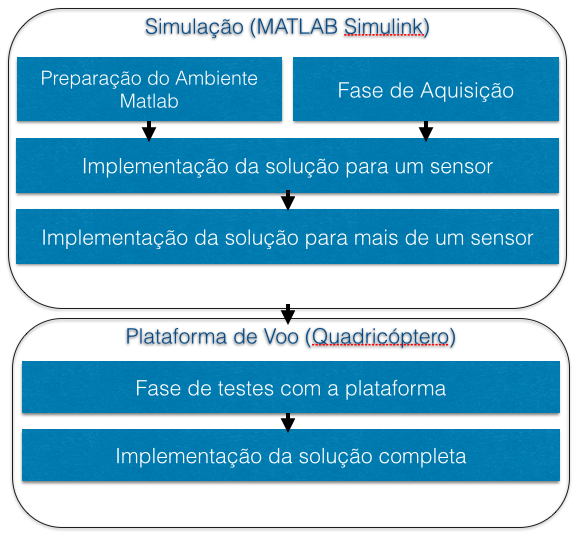
\includegraphics[scale=0.5]{img/fluxo.png}
	\caption{Estratégia de implementação}
	\label{fig:Fluxo}
\end{figure}

\newpage


\section{Cronograma} 
\label{sec:crono}
Para facilitar a compreensão do projeto, optou-se por dividir o trabalho em módulos que seguirão o cronograma abaixo.
\begin{figure}[h]
	\centering
		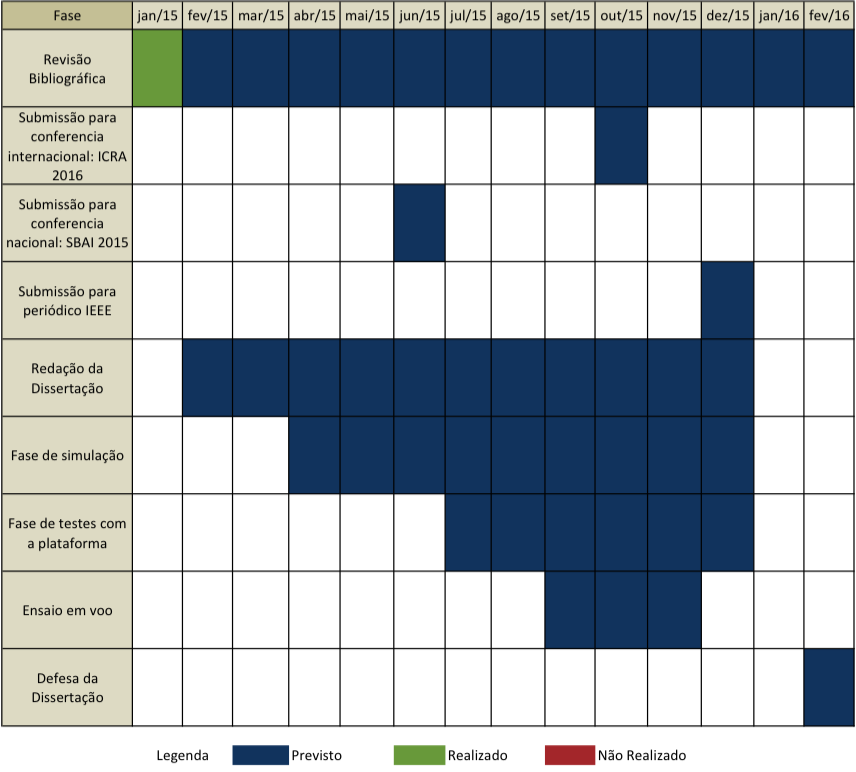
\includegraphics[scale=0.4]{img/cronograma.png}
	\caption{Cronograma físico.}
	\label{fig:cronograma}
\end{figure}

\newpage

\section{Viabilidade da proposta}
\label{sec:viabilidade}

A viabilidade desta proposta depende da obtenção dos itens necessários para implementação e testes do método. A partir dos componentes e software necessários descritos nas seções \ref{subsec:hardware} e \ref{subsec:software}, foi feito um levantamento dos itens já disponíveis para teste e os que necessitam ser adquiridos. A seguir está a listagem dos itens e suas disponibilidades no Laboratório de Robótica RoboIME.

\begin{itemize}
	\item
	Plataforma de voo:  O laboratório dispõe de quatro quadricópteros para teste, com aproximadamente 45cm de diâmetro, com capacidade de carga suficiente para embarcar um minicomputador e sensores ultrassônicos.
	\item
	Minicomputador: Estão disponíveis dois minicomputadores Raspberry PI modelo B com processador de 700MHz, 512MB de memória, duas saídas USB e portas de rede Ethernet para testes.
	\item
	Sensores ultrassônicos: Inicialmente, serão utilizados sensores ultrassônicos modelo \underline{XXXXX} já adquiridos que terão suas capacidades avaliadas. Caso haja a necessidade de aquisição, são itens de baixo custo e facilmente encontrados no mercado brasileiro.
	\item
	MatLab Simulink: Usaremos o Matlab R2013a com Simulink, versão para estudante que possui todas as ferramentas necessárias para simulação do problema. 

\end{itemize}

A princípio, estes itens serão suficientes para o inicio dos trabalhos e atestam a viabilidade da proposta. Outra alternativa, que poderá ser avaliada, é a utilização de um sensor de varredura a laser em miniatura Hokuyo-URG. Este está em fase de aquisição pelo laboratório e poderia substituir os sensores ultrassônicos, caso apresente um melhor desempenho.

\newpage

\section{Resultados Esperados}
\label{sec:resultados}
 Para avaliação do método, foram estipuladas três missões que o quadricóptero precisa ser capaz de realizar. Em todas, ele deverá evitar a colisão, mantendo uma distância segura dos obstáculos. Cada missão avalia o método em diferentes situações e estão descritas a seguir.
 
 \noindent\textbf{Missão 1: Manter sua posição enquanto estabilizado e nenhuma saída}
 
 O quadricóptero será estabilizado e cercado, não tendo caminho possível de ser realizado enquanto o piloto executa comandos de controle. O \textit{input} do controle será ignorado, ou seja, qualquer comando realizado pelo piloto será desprezado e a plataforma manterá sua posição. Um esboço da situação pode ser visualizado na Figura \ref{fig:missao1}. Esta missão irá avaliar se o método consegue evitar os obstáculos em todas direções $(x,y)$.
 
 \begin{figure}[h]
 	\centering
 	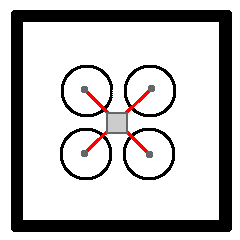
\includegraphics[scale=0.5]{img/missao1.png}
 	\caption{Missão 1. Veículo cercado e estabilizado}
 	\label{fig:missao1}
 \end{figure}  
 
 \noindent\textbf{Missão 2: Desviar de um obstáculo estático a frente}
 
 Nesta missão, o quadricóptero será conduzido a uma velocidade de aproximadamente \underline{$2m/s$} através de uma trajetória retilínea em um ambiente \textit{indoor} enquanto depara-se com um obstáculo a frente. Ele irá realizar um desvio pela lateral do obstáculo. Será escolhido o lado que exija o menor desvio possível (Figura \ref{fig:missao2}). Esta missão irá avaliar se o método consegue desviar a trajetória do quadricóptero, perante um obstáculo, quando em movimento.

\begin{figure}[h]
	\centering
	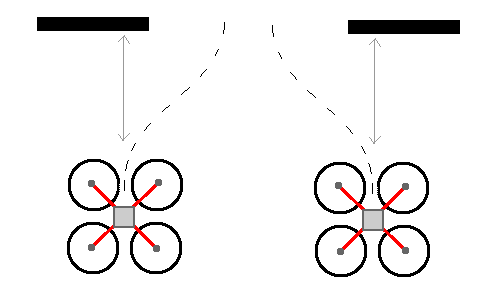
\includegraphics[scale=0.5]{img/missao2.png}
	\caption{Missão 2: Veículo em movimento com obstáculo a frente. Um desvio à direita (esquerda) e um desvio à esquerda (direita)}
	\label{fig:missao2}
\end{figure}  
 
 \noindent\textbf{Missão 3: Realizar uma trajetória segura num ambiente com vários obstáculos} 
  
 Por fim, o quadricóptero será conduzido a uma velocidade de aproximadamente $2m/s$ por um trajeto completo, com diversos obstáculos em posições variadas, e ele deverá ser capaz de terminá-lo sem colisões. O objetivo desta missão é avaliar a eficácia e o benefício do método simulando a condução de um quadricóptero num ambiente complexo de difícil pilotagem. A Figura \ref{fig:missao3} ilustra o mapa do ambiente a ser utilizado com as setas indicando o início e o fim do trajeto.
  
  
 \begin{figure}[h]
 	\centering
 	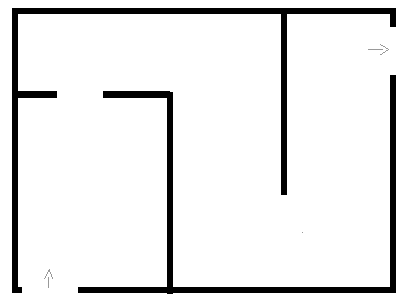
\includegraphics[scale=0.4]{img/missao3.png}
 	\caption{Missão 3: Trajeto completo num ambiente com obstáculos}
 	\label{fig:missao3}
 \end{figure}  
  
\newpage

\section{Conclusão}
\label{sec:conclusao}

O advento da utilização dos VANT's, mais especificamente os quadricópteros, em ambientes restritos, trazem a tona a necessidade de controlar o desvio de obstáculo de forma automática. Este é um tema que tem merecido atenção na área de robótica e nossa proposta visa explorá-lo com medições de sensores em tempo real, auxiliando o controle do veículo. Com esse enfoque, nossa proposta é viável e poderá ser utilizada em uma variedade de aplicações na área de defesa.  Além disso, a solução, uma vez construída, será o módulo de desvio de obstáculos da plataforma VANT-IME, que está em fase de concepção no Laboratório RoboIME.

\newpage

\bibliographystyle{abbrv}
\bibliography{Dissertacao} 

\newpage

\begin{center}
\_\_\_\_\_\_\_\_\_\_\_\_\_\_\_\_\_\_\_\_\_\_\_\_\_\_\_\_\_\_\_\_\_\_\_\_\_\_\_\_\_\_\_\_\_\_\_\_\_\_\_ \\

Bruno da Silva Giovanini (ED 14106) \\Aluno \\ 
 
\hspace{4cm}
\\


\_\_\_\_\_\_\_\_\_\_\_\_\_\_\_\_\_\_\_\_\_\_\_\_\_\_\_\_\_\_\_\_\_\_\_\_\_\_\_\_\_\_\_\_\_\_\_\_\_\_\_ \\
Paulo Fernando Ferreira Rosa, Ph.D \\Orientador \\ 

\hspace{4cm}
\\


\_\_\_\_\_\_\_\_\_\_\_\_\_\_\_\_\_\_\_\_\_\_\_\_\_\_\_\_\_\_\_\_\_\_\_\_\_\_\_\_\_\_\_\_\_\_\_\_\_\_\_ \\
Maj Ronaldo Moreira Salles, Ph.D \\Coordenador de Pós-Graduação \\

\hspace{4cm}

\end{center}
Concordo com a presente Proposta de Dissertação e declaro que as necessidades para sua execução serão garantidas pelo departamento. \\
IME, em \today
 \hspace{4cm}
 \\
 \\
 \\
 \\
 
\begin{center}
\_\_\_\_\_\_\_\_\_\_\_\_\_\_\_\_\_\_\_\_\_\_\_\_\_\_\_\_\_\_\_\_\_\_\_\_\_\_\_\_\_\_\_\_\_\_\_\_\_\_\_\_\_\_\_\_\_\_\_ \\
Antonio Carlos Freire de Almeida, Ten Cel QEM, \\
CHEFE SE/8
\end{center}


\end{document}